\documentclass[12pt, a4paper]{article}
\usepackage{amsmath,amssymb,mathrsfs,fancyhdr,syntonly,lastpage,hyperref,enumitem,graphicx,float}
\usepackage{booktabs}
\usepackage{tabu}
\usepackage[table,xcdraw]{xcolor}
\usepackage[english]{babel}
\usepackage[utf8]{inputenc}
\usepackage{amsmath}
\usepackage{graphicx}
\usepackage[colorinlistoftodos]{todonotes}
\usepackage[toc,page]{appendix}
\usepackage{caption}
\usepackage{subcaption}

\title{A Bayesian approach to estimate time of maximal ``greenness" in Tropical Evergreen India}

\author{Manju M. Johny}

\date{\small \today}

\begin{document}
\maketitle


\section{Introduction }
\qquad The behavior of natural vegetation is known to entrain to the cyclical rhythm of seasons. For example, cherry blossoms consistently bloom in the spring, and hoards of watermelon arrive at the supermarket in the summer followed  
by squashes and pumpkins in the fall. In this regard, a statistical model to estimate the optimal periods of growth for particular crops in a given region would be greatly beneficial to the agriculture industry. 

The MERIS Terrestrial Chlorophyll Index (MTCI) is a satellite-measured index of chlorophyll content invaluable in studying the phenology of vegetation. The chlorophyll index of an area is a measure of the ``greenness" of the region of interest, with large MTCI values corresponding to greater ``greenness." In this project, we explore MTCI of the Indian sub-continent measured over a span of 4 years. In particular, we limit our analysis to the phenology of one pixel from the available 50 x 50 matrix describing the area spanning the Indian sub-continent. Figure 1 shows a plot of the MTCI values over time for the given pixel of interest. The cyclical pattern in ``greenness" is apparent in this plot -- with 1 distinct peak of ``greenness" in each of the 4 periods present. Accordingly, we utilize a Bayesian approach to determine the times at which maximum ``greenness" is achieved per period.    

\section{Data}
\qquad This project uses Level 3 Medium Resolution Imaging Spectrometer (MERIS) Terrestrial Chlorophyll Index (MTCI) data provided by NERC Earth Observation Data Center. MERIS operates at a spatial resolution of 4.6 km \cite{dash}. MTCI is calculated, using the standard MERIS band settings, as the ratio of differences in reflectance between spectral bands 10 ($\lambda = 753.75 nm$) and 9 ($\lambda = 708.75 nm$), and spectral bands 9 ($\lambda =  708.75 nm$) and 8 ($\lambda =  681.25 nm$) \cite{Jeg}. 

\begin{equation}
MTCI = \frac{R_{10} - R_{9}}{R_{9} - R_{8}}
\end{equation}

MTCI measurements were taken, in 8 day intervals between 2004 and 2007, of the area spanning the Indian sub-continent \cite{dash}. The MTCI measurements are arranged into 50 x 50 matrices where each cell gives the MTCI value of a particular pixel or area of land. The data set is composed of 4 different files for each year. Each file contains a list of matrices, each of dimension 50 x 50, arranged chronologically by time of measurement. All together, the 4 files contain 184 matrices of dimension 50 x 50. Additionally, we used information classifying the pixels in the matrix by the predominant vegetation type of the area. This information about vegetation type is summarized by another matrix, where each cell represents the predominant vegetation type of the corresponding pixel in our MTCI data set. There are 47 possible vegetation types, each of which are represented by numbers 0 through 46. For this project, we focus on just one pixel belonging to the vegetation type ``Tropical Evergreen". Our pixel of interest is the $5^{th}$ element of the matrix (row = 1, col = 5). Figure 1 shows a plot of the MTCI values by time for the pixel of interest.                        

\section{Methods}

\subsection{Model Rationale}
\qquad Figure 1, the plot of MTCI values over time for our pixel of interest, exhibits obvious sinusoidal behavior. We employ Bayesian sinusoidal regression to model the cyclical behavior of the pixel's MTCI values over time. There are 4 distinct peaks in the total span of 4 years. Hence, the period appears to be the length of 1 year. For simplicity, we consider a fixed period in this project defined as the length of one tropical year per 8 days.
\begin{equation}
\omega = \frac{365.2421897}{8} = 45.6553
\end{equation}
Along with the sinusoidal terms, we will include an intercept term and a linear trend term in the model.

\subsection{Model}
\qquad For our pixel of interest, let $y_{t}$ be the MTCI value at the $t^{th}$ time point. Let t, ranging from 1 through 184, be the time point at which each MTCI measurement was taken. Recall that t is measured every 8 days. Additionally, we also assume that $y_{t}$ are distributed independently.
\textbf{\\ Data Model}\\
\text{For given time period,} t = \{1,2,..,184\}:
\begin{equation}
\begin{split}
y_{t}
& \overset{ind}{\sim} N\big(\mu_{t}, \tau^2\big) 
\end{split}
\end{equation}
\begin{equation}
\begin{split}
\mu_{t}
& = \beta_{0} + \beta_{1}t + \beta_{2}\text{cos}\bigg(\frac{2\pi t}{45.6553}\bigg) + \beta_{3}\text{ sin}\bigg(\frac{2\pi t}{45.6553}\bigg)
\end{split}
\end{equation}
\textbf{Priors}
\begin{equation}
\begin{split}
\tau
& \sim Ca^{+}\big(0, 0.04)\\
\beta_{0}
& \sim U\big(0, 10)\\
\beta_{1}
& \sim U\big(-10, 10)\\
\beta_{2}
& \sim U\big(-10, 10)\\
\beta_{3}
& \sim U\big(-10, 10)\\
\end{split}
\end{equation}
\qquad Valid MTCI values range from 1 to 6 \cite{dash}. The uniform priors on the $\beta$ parameters were chosen such that they allowed coverage of valid ranges of MTCI values. The intercept term, $\beta_0$'s uniform prior has sufficient density over the possible values for the intercept (values between 1 and 6). Similarly, $\beta_1$'s uniform prior has sufficient density over the possible values for the linear trend term, including both positive and negative trends. Consider the trigonometric equivalence
\begin{equation*}
\begin{split}
\beta_{2}\text{cos}\bigg(\frac{2\pi t}{45.6553}\bigg) + \beta_{3}\text{sin}\bigg(\frac{2\pi t}{45.6553}\bigg) &= A \text{cos}\bigg(\frac{2\pi t}{45.6553} - \delta \bigg)\\
\text{where the amplitude, } A &= \sqrt{\beta_{2}^{2}+\beta_{3}^{2}}.
\end{split}
\end{equation*}
Plausible values for the amplitude are confined between 0 and 5 based on the valid ranges of MTCI values. Thus, the uniform priors on $\beta_{2}$ and $\beta_{3}$ were chosen such that they have sufficient density over possible values of the amplitude. The intervals for the $\beta$ parameters' uniform priors are wider than necessary. We could have also chosen more narrow intervals for the priors on each of the $\beta$ parameters and still maintained sufficient coverage over plausible values. Lastly, a half Cauchy prior was chosen as a diffuse prior for the standard deviation, $\tau$. Since all of the priors used were proper, we have assurance of posterior propriety.

\subsection{Model Fitting}   
\qquad JAGS was used with the rjags package to generate samples from the posterior distribution of the parameters. A 3 chain MCMC was run for 10,000 iterations with a burn-in period of 5,000 iterations using R's default starting values. Ultimately, this culminated in 30,000 MCMC samples generated for the $\beta$ and $\tau^2$ parameters.  The potential scale reduction factors for the parameters, given in Appendix: Table A.1, were all 1. Additionally, the trace plots, shown in Appendix: Figure A.1, indicated well mixed chains. Based on the potential scale reduction factors and the trace plots, there was no indication of lack of convergence in the Markov Chains. Figure 3 shows a comparison of 19 replications from the posterior predictive distribution of y, and our observed data. A comparison of the replications to our observed data shows no indication of lack of fit in our model.
\section{Results}
\qquad We were able to obtain posterior distributions for the unknown parameters along with their estimates using MCMC. The posterior distribution for the $\beta$ and $\tau^2$ parameters are shown in Figure 4. Additionally, the posterior medians and $95\%$ credible intervals for each of the parameters are reported in Table 1. For each iteration. the resulting posterior $\beta$ parameters were used to calculate $\mu_{t}$ according to Eq (4). The $95\%$ credible intervals and posterior median for the marginal posterior of $\mu_{t}$ is shown in Figure 2.

In Figure 2, there are 4 distinct peaks in $\mu_{t}$, where each peak is confined to its respective period ($\omega$ = 45.6553 time points). In order to answer the scientific question of interest, we create credible intervals for the time points at which each of these peaks appear. For each of the 30,000 posterior samples, the time point corresponding to maximum $\mu_{t}$ within a period was determined. So, each iteration gave 4 distinct time points per cycle at which maximum $\mu_{t}$ was reached -- lets call these values peaktime$_{1}$, peaktime$_{2}$, peaktime$_{3}$ and, peaktime$_{4}$. From these peaktimes in each of the 30,000 samples, we were able to create 95$\%$ credible intervals for peaktime. These credible intervals are summarized in Table 2. Additionally, we may be interested in peaktime as measured from the end of the previous cycle. The posterior $95\%$ credible intervals for this information is summarized in Table 3.      
\section{Discussion}
\qquad The objective of this project was to identify the time points at which maximum ``greenness" occurred per cycle. We estimated these values by creating posterior credible intervals for peaktimes. Peaktimes are defined as the time points at which maximum posterior $\mu_{t}$ is achieved per cycle. We obtained estimates for each of the four peaktimes as summarized in Table 2. The posterior median peaktimes, over the four year period, were at the $29^{th}$, $75^{th}$, $121^{st}$, and $166^{th}$ time points. The 95$\%$ credible intervals around the posterior medians are tight, varying at most by 1 time point from the median. Additionally, we may further be interested in the peaktimes as measured from the end of the previous period. The posterior median peaktimes, at each of the four periods, occurred respectively at $29$, $29$, $30$, and $29$ time points after the end of the previous period. The 95$\%$ credible intervals for peaktimes, for all four periods, are between 29 and 30 time points after the end of the previous period. Converted to days, these time points correspond to 232 and 240 days respectively. The similarity of peaktimes over the four periods shows consistency among the times at which maximum ``greenness" is achieved year to year from 2004 to 2007. 
\section{Improvements and Future Work}
\qquad For simplicity, we assumed a fixed period defined as the length of 1 tropical year per 8 days. However, the true period need not be exactly that length. A better approach may have been to put a prior on the period, $\omega$, and estimate it along with the other parameters. Additionally, the phenology of the Indian sub-continent is known to house diverse land types, some of which exhibit distinct phenological behaviors. For example, certain land types have more than one growing season -- giving multiple peaks in MTCI values per year. It could be interesting to build a hierarchical model, grouping together pixels by vegetation type. Additionally, we could have also approached this problem from a dynamic linear modeling perspective. This project, while an illuminating first step, merely scratches the surface of greater statistical and phenological understanding that could be fostered from this data set.  

\section{Figures}
\begin{figure}[H]
\centering
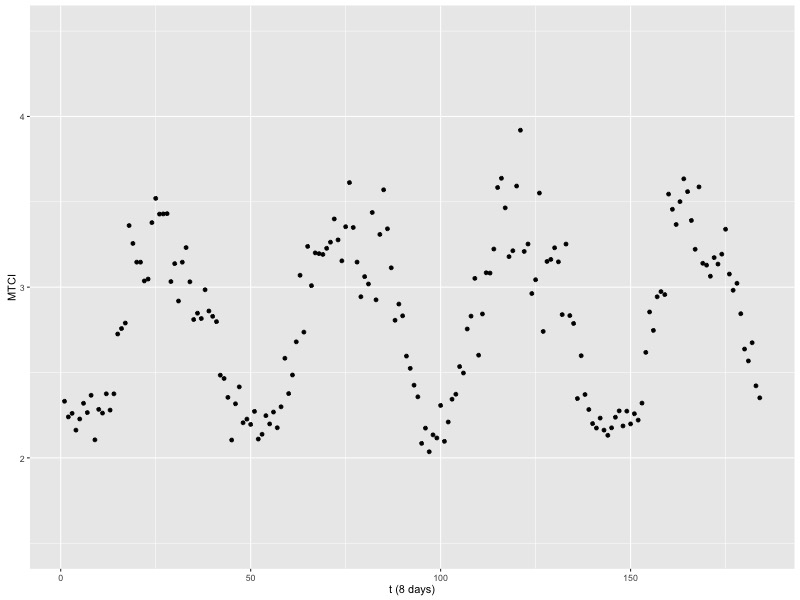
\includegraphics[width=0.7\linewidth]{projectfig0.jpeg}
\caption{\small Plot of MTCI values over time for the pixel of interest.}
\end{figure}

\begin{figure}[H]
\centering
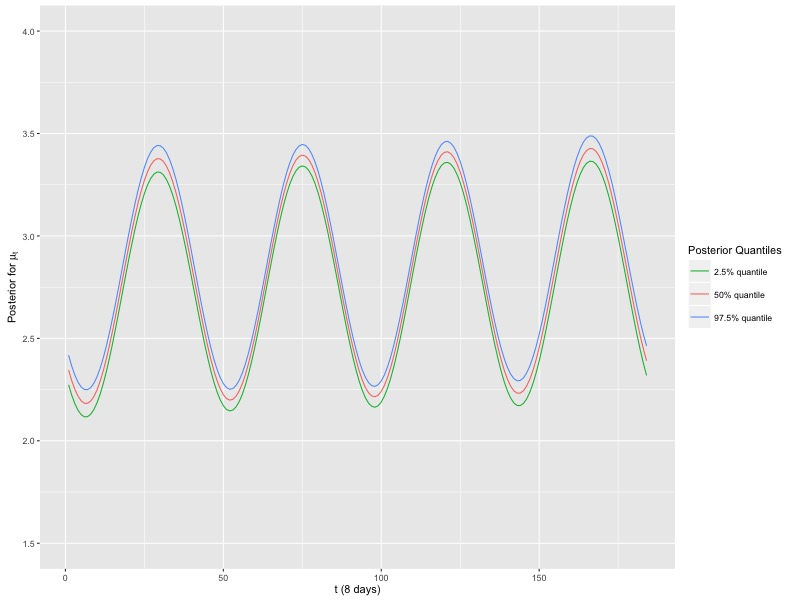
\includegraphics[width=0.85\linewidth]{projectfig2.jpeg}
\caption{\small Quantiles for the posterior distribution of $\mu_{t}$. The red line indicates the posterior median for $\mu_{t}$. A 95$\%$ credible interval for $\mu_{t}$ is contained in the area between the green line ($2.5^{th}$ quantile) and blue line ($97.5^{th}$ quantile).}
\end{figure}

\begin{figure}[H]
\centering
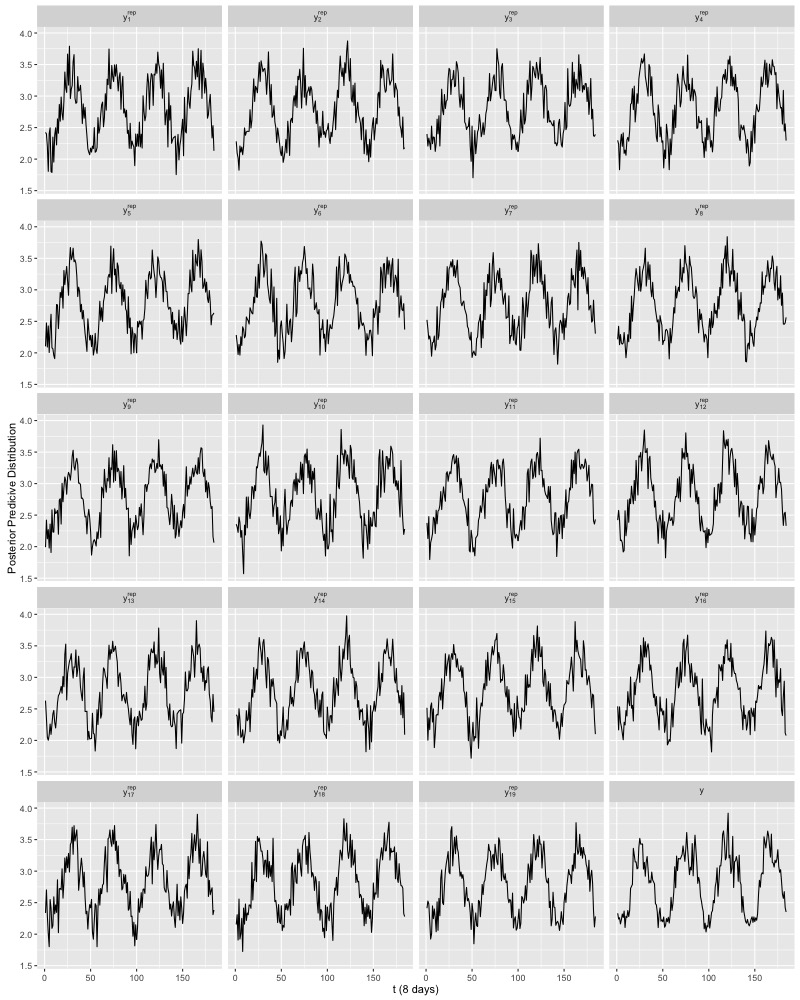
\includegraphics[width=1\linewidth]{projectfig3.jpeg}
\caption{\small Comparison of 19 replications from the posterior predictive distribution of y ($y^{rep}$), and observed data (y).}
\end{figure}



\begin{figure}[H]
\centering
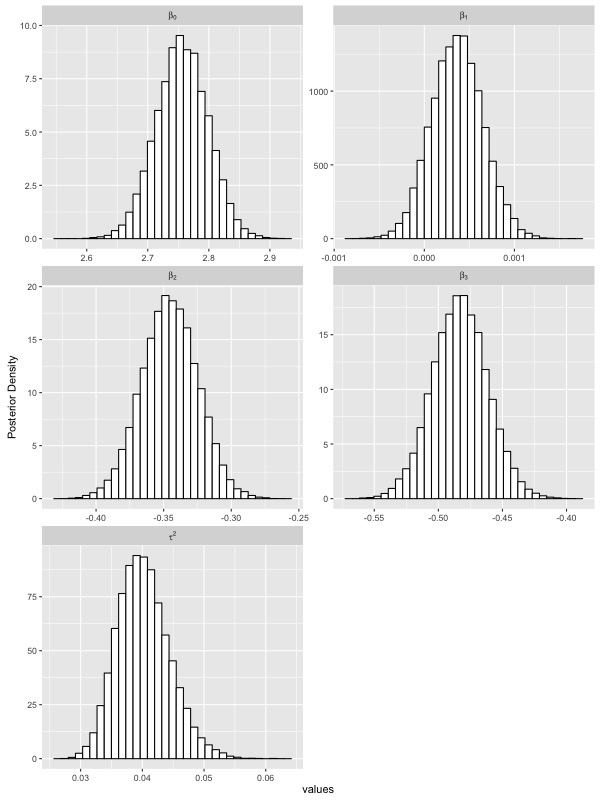
\includegraphics[width=1\linewidth]{projectfig1.jpeg}
\caption{\small Histograms of the posterior distribution of $\beta_{0},\beta_{1}, \beta_{2},\beta_{3}, \tau^{2}$ based on 30,000 posterior samples generated using MCMC.}
\end{figure}



\section{Tables}
\begin{table}[H]
\centering
\caption{\small Summaries of the posterior distributions of $\beta$ and $\tau^{2}$ parameters. The posterior median, and central $95\%$ posterior credible intervals for each parameter is shown below.}
\label{my-label}
\begin{tabu} to \textwidth {Xlc}
\toprule
& Posterior median  & 95$\%$ posterior credible interval \\ \midrule
$\beta_{0}$ & 2.76   & [2.67, 2.84]     \\
$\beta_{1}$ & 0.0004 & [-0.0002, 0.0009]   \\
$\beta_{2}$ & -0.35  & [-0.39, -0.30]    \\
$\beta_{3}$ & -0.48  & [-0.53, -0.44]    \\
$\tau^{2}$  &  0.040     & [0.033, 0.049]       \\ \bottomrule
\end{tabu}
\end{table}

\begin{table}[H]
\centering
\caption{\small Summaries of the posterior distributions of peaktimes. ``peaktime$_{p}$" represents the time point at which $\mu_{t}$ is maximized over the $p^{th}$ period. The posterior median, and central $95\%$ posterior credible interval for peaktimes at each of the 4 periods is shown below.}
  \label{}
  \begin{tabu} to \textwidth {Xlc}
  \toprule
  & Posterior median  & 95$\%$ posterior credible interval \\ \midrule
  peaktime$_{1}$ & 29                & [29, 30]       \\
  peaktime$_{2}$ & 75                & [75, 76]       \\
  peaktime$_{3}$ & 121               & [120, 121]      \\
  peaktime$_{4}$ & 166               & [166, 167]      \\ \bottomrule
  \end{tabu}
  \end{table}
  
  \begin{table}[H]
  \centering
  \caption{\small Summaries of the posterior distributions of peaktimes as measured from the end of the previous period. ``peaktime$_{p}$" represents the time point (starting from the end of the previous period) at which $\mu_{t}$ is maximized over the $p^{th}$ period. The posterior median, and central $95\%$ posterior credible interval for peaktimes at each of the 4 periods is shown below.}
\label{}
\begin{tabu} to \textwidth {Xlc}
\toprule
& Posterior median  & 95$\%$ posterior credible interval \\ \midrule
peaktime$_{1}$ & 29              & [29, 30]       \\
peaktime$_{2}$ & 29              & [29, 30]       \\
peaktime$_{3}$ & 30              & [29, 30]      \\
peaktime$_{4}$ & 29              & [29, 30]      \\ \bottomrule
\end{tabu}
\end{table}

\section{Appendix}
\renewcommand\thetable{A.1}
\begin{table}[H]
\centering
\caption{\small Potential scale reduction factors for estimated parameters, $\beta_{0}$, $\beta_{1}$, $\beta_{2}$, $\beta_{3}$, $\tau^{2}$, as calculated using the coda package. Point estimates and upper confidence limits of the potential scale reduction factors are reported.}
\label{}
\begin{tabu} to \textwidth {Xlc}
\toprule
& Point estimate  & Upper confidence limit \\ \midrule
$\beta_{0}$ & 1              & 1       \\
$\beta_{1}$ & 1              & 1       \\
$\beta_{2}$ & 1              & 1      \\
$\beta_{3}$ & 1              & 1      \\
$\tau^{2}$ & 1              & 1      \\ \bottomrule
\end{tabu}
\end{table}
\renewcommand\thefigure{A.1}
\begin{figure}[H]
\centering
\begin{subfigure}{.5\textwidth}
\centering
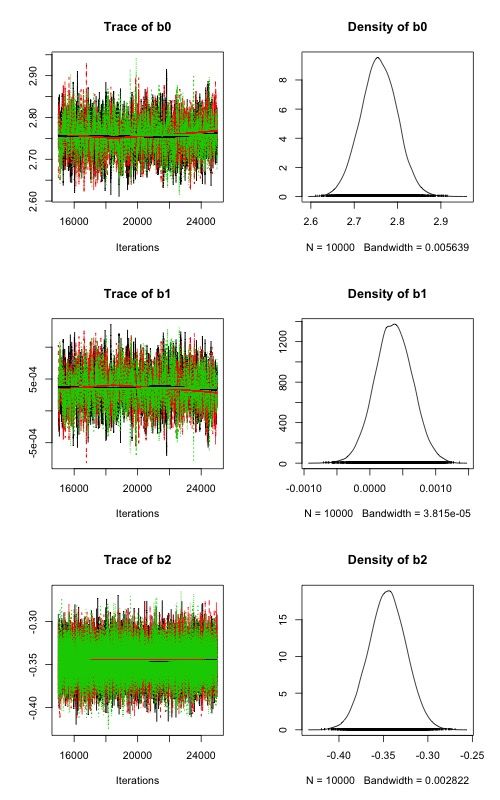
\includegraphics[width=1\linewidth]{Afig1.jpeg}
\end{subfigure}%
\begin{subfigure}{.5\textwidth}
\centering
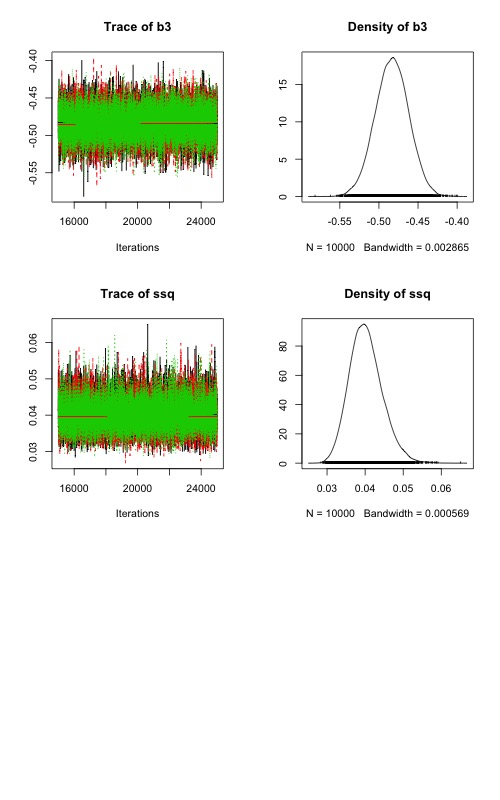
\includegraphics[width=1\linewidth]{Afig2.jpeg}
\end{subfigure}
\caption{\small Trace plots and densities of the estimated parameters. $\beta_{0}$, $\beta_{1}$, $\beta_{2}$, $\beta_{3}$, and $\tau^{2}$ are represented as ``b0", ``b1", ``b2", ``b3", and ``ssq" respectively in the plots.}
\end{figure}
  
  
\bibliographystyle{plain}
\bibliography{project} 
  
\end{document}